\chapter{Introdução}\label{Introdução}

Neste capítulo é apresentada a motivação do presente estudo, assim como seus objetivos e sua organização.

\section{Motivação}

O comportamento do motorista afeta em grande parte a segurança no transito \cite{evans2004traffic}, estima-se que 856,000 acidentes de estrada ocorrem anualmente, sendo 74\% deles em países subdesenvolvidos (\citeauthor{worldhealthorganization2018}, \citeyear{worldhealthorganization2018}). Em 2004, os acidentes de trânsito representavam a nona mais importante causa de morte no mundo, com 1,2 milhão de vítimas \cite{bacchieri2011acidentes} A OMS estima que em 2030 subirão para a quinta posição. Felizmente, estudos mostram que é possível adaptar o comportamento do condutor de forma a aumentar a segurança, diminuir o consumo de combustível e as emissões de gases dos veículos \cite{goldberg2000} \cite{almazan2013full}. Em vista disso, a Análise de Perfil de Motorista (APM) se apresenta como uma forma de melhorar o comportamento do motorista, levando ele a uma condução mais segura e consciente. (\citeauthor*{zheng2016unsupervised}, \citeyear{zheng2016unsupervised}; \citeauthor{castignani2015driver},  \citeyear{castignani2015driver})

A APM consiste na coleta de dados de condução através de diversos sensores e em seguida a aplicação de um modelo computacional a fim de gerar pontos ou uma classificação que caracterize a forma de dirigir do motorista (\citeauthor*{eren2012estimating}, \citeyear{eren2012estimating}). Nesse sentido são apresentados diversos estudos que analisam hábitos de direção. Grande parte deles utilizam uma vasta gama de sensores do próprio veículo, tal como sensores externos (câmeras, microfones e radares). 
smartfones modernos oferecem sensores adequados para coletar dados para a análise de perfil de condutor \cite{junior2017driver}. Trabalhos anteriores (**citar trabalhos**) demonstram a alta correlação entre as medições de sensores embarcados em dispositivos smartfones e caixas telemáticas instaladas fixamente nos veículos. Embora haja espaço para desenvolvimento e melhorias, os smartfones se provaram uma forma conveniente de se instrumentar a coleta de dados em um veículo.

Em linhas gerais a APM tem se tornado cada vez mais relevante. \citeauthor{junior2017driver} \cite{junior2017driver} destaca que telemática de seguros, particularmente, tem se apropriado da tecnologia de forma a  tornar mais barato o valor da franquia para motoristas com boas pontuações, ao invés de usar apenas estatísticas que dizem respeito a grupos (e.g, idade, sexo, estado civil).

É observada na literatura diversos trabalhos (\cite{Paefgen:2012:DBA:2406367.2406412},\cite{eren2012estimating}) que utilizam alguma especie de fusão de sensores para classificar a corrida de motoristas. \citeauthor{araujo2012driving} criou um Aplicativo com o objetivo de conscientizar os motoristas no que diz respeito ao consumo de combustível. Para tal, se utilizam os sensores do smartfone(GPS) e o estado do veículo(velocidade, combustível, aceleração, etc.), processados através de um algoritmo que utiliza lógica fuzzy. Em seguida o consumo é comparado com com métricas providas pela montadora do carro. Os resultados preliminares mostram um potencial de redução do consumo de combustível e a mudança no comportamento do motorista.

Outro trabalho \citep{chen2015d} propõem a identificar movimentos de direção agressivos, através da análise dos sensores de GPS e acelerômetro de um dispositivo smartfone. A princípio, os eixos do carro e do aparelho são alinhados manualmente, fazendo sentido dos dados observados pela captura de sensores. Para detecção de eventos, o algoritmo compara o desvio padrão da assinatura e a média, com alguns limiares, de forma a observar o início de um evento. Depois de iniciado o algoritmo monitora as médias e os desvios padrões nos eixos para constatar que o evento chegou ao fim. Em seguida a janela armazenada alimenta uma SVM que é capaz de detectar e distinguir com 95.36\% de acurácia 6 eventos de direção.

\begin{figure}
    \centering
    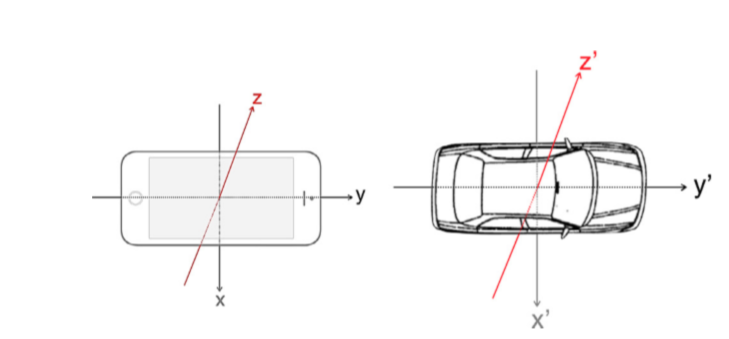
\includegraphics[width = 150mm]{Figuras/celularcarro.PNG}
    \caption{Sistema de Coordenadas do Celular Alinhado com Sistema de Coordenadas do Veículo\\Fonte: \citeauthor{vlahogianni2017driving} (\citeyear{vlahogianni2017driving})}
    \label{fig:celularCarroAlinhados}
\end{figure}{}


No entanto, em um caso prático, dificilmente o dispositivo móvel se encontra com o eixo dos seus sensores alinhados com o carro (conforme exemplificado pela Figura \ref{fig:celularCarroAlinhados}). Nesse caso, empobrece-se a analise e quantidade de informação que se pode extrair de uma viagem, no que tange ao comportamento do motorista. Diversos trabalhos que buscam realizar a APM através dos dados coletados através de dispositivos smartfones, recorrem ao alinhamento manual do aparelho com o carro ou a transformação de eixos para o sistema de coordenadas global. O primeiro método possui como limitante, a variabilidade da posição do dispositivo em um caso real de uso.

O segundo método deve lançar mão do magnetômetro embarcado no dispositivo. Esse sensor aparece cada vez mais nos dispositivos ao longo dos anos, porém de acordo com a Tabela \ref{tab:aparelhosMaisVendidos}, 50\% dos aparelhos mais vendidos em 2018 não possuíam o magnetômetro, o que pode se tornar um gargalo para adoção ampla do método. Em suma, o magnetômetro funciona como uma espécie de bussola, devido a capacidade do sensor de captar tanto campos magnéticos locais como o campo magnético terrestre. Nesse sentido, o sensor é utilizado em conjunto com o sensor de gravidade - um sensor virtual, que é obtido através de uma filtragem de baixa no acelerômetro -, com o objetivo de migrar o sistema de coordenadas local do celular, para um sistema de coordenadas global. No entanto, é mostrado na literatura(**citar**) que a sensibilidade do magnetômetro é alta, e suas medições são alteradas na presença de pequenos campos magnéticos e objetos metálicos. Uma vez que a gama de eletro-eletrônicos embarcados em um veículo só tende a aumentar, devido a maior interconectividade entre os sistemas do carro, a medição do campo captado por esse sensor se torna cada vez mais imprecisa. Outro aspecto dessa problemática advém de que um sistema de coordenadas global diz pouco a respeito da dinâmica veicular observada no carro.


\begin{table}[]
\centering
\caption{Presença do Magnetômetro nos Aparelhos mais vendidos de 2018 }
\label{tab:aparelhosMaisVendidos}
\begin{tabular}{lc}
\textbf{Aparelho} & \textbf{Possui Magnetômetro} \\ \hline
Moto G6 Plus & sim \\
Moto X4 & não \\
Moto Z2 Play & sim \\
Galaxy S8 & sim \\
Galaxy J7 Prime 2 & não \\
Galaxy J5 Prime & não \\
Motorola Moto G5s plus & não \\
Galaxy J5 Pro & sim \\
Galaxy J7 Pro & sim \\
Motorola Moto G5s & não \\ \hline
\multicolumn{2}{l}{Fonte: Próprio Autor com base em dados disponibilizados pelos Fabricantes}
\end{tabular}
\end{table}




\section{Objetivos}

Nesse contexto, a contribuição deste trabalho é dupla. Primeiramente por derivar uma forma de se generalizar a captura de movimentos do telefone, utilizando apenas o giroscópio e o acelerômetro, sensores que são comuns a maioria dos smartfones. Para tal, o trabalho busca apresentar um método de transferência de coordenadas similar ao encontrado na literatura, no entanto com a vantagem de ser robusto a partida no plano inclinado e por realizar a calibração nos primeiros instantes de movimento. Ou seja, quando o carro parte do plano reto ou inclinado, a calibração se dá de forma praticamente instantânea.

Em segundo lugar, o trabalho apresenta sistema de coordenadas que é compatível com a dinâmica veícular, assim podendo inclusive derivar informações relevantes a respeito dos padrões de direção observando limiares já conhecidos de curva, aceleração e desaceleração.

\section{Contextualização}

Nesta seção serão contextualizados alguns conceitos associados à APM. O primeiro a ser abordado é a telemática. 

A telemática consiste no uso de computação, monitoramento por sensores e tecnologias de comunicação para prover serviços em um meio automotivo. Alguns serviços de telemática incluem navegação, diagnóstico remoto, gestão de frota, segurança, percepção de contexto e comércio mobile.

Nesse contexto a navegação compreende um dos serviços de telemática mais prevalentes; onde, tipicamente, envolve um sistema de posicionamento global (GPS) e um mapa, integrado com uma base de dados, que proporciona direções para o motorista. No ambiente automotivo, o sinal de GPS pode ser afetado por diversos fatores, como: Interferência dos proprios eletrônicos no veículo, local de posicionamento da antena, performance da antena e obstruções de sinal. De forma a melhorar a disponibilidade e a performance de sistemas de navegação, o dispositivo GPS é combinado, com alguns sistemas de navegação inercial ou sensores Dead Reckoning (DR) como observado em \cite{ochieng2003integration} e \cite{cho2006robust}.

Atualmente, os smartfones são equipados com diversos sensores utilizados em soluções APM. Como é o caso do sensor de GPS e acelerômetro, giroscópio tri-axial (lateral, longitudinal e vertical). O GPS fornece a localização e velocidade do dispositivo. O acelerômetro mede a intensidade da aceleração causada pelo movimento do telefone. O giroscópio mede o quanto o dispositivo está sendo rotacionado em torno dos eixos.

No que diz respeito ao aspecto da segurança, a telemática veicular combina sensoriamento com comunicações sem fio, de forma a detectar e evitar situações inseguras ao se dirigir o veículo. Nesse trabalho, por exemplo \cite{eren2012estimating}, os autores foram capazes de utilizar o acelerômetro, giroscópio e o magnetômetro presente em um smartfone, para estimar se o comportamento do motorista no trânsito era seguro ou não.

\section{Organização do Trabalho}

No \autoref{RevisãoBibliográfica} serão apresentados os fundamentos teóricos que embasam todo o desenvolvimento deste trabalho, assim como alguns trabalhos científicos que servirão de comparação para os resultados.


